\documentclass[11pt,conference]{IEEEtran}

\usepackage[latin1]{inputenc}
\usepackage{amsmath}
\usepackage{amsfonts}
\usepackage{amssymb}
\usepackage{graphicx}
\usepackage{hyperref}

\usepackage{listings}
\usepackage{subcaption}
%\usepackage{subfig} % make it possible to include more than one captioned figure/table in a single float
\usepackage{algorithm} 
\usepackage{algpseudocode}
\usepackage[font=small]{caption}

\title{UrDHT: A Unified Model for Distributed Hash Tables}



\author{\IEEEauthorblockN{Andrew Rosen \qquad Brendan Benshoof \qquad Robert W. Harrison \qquad Anu G. Bourgeois}
	\IEEEauthorblockA{Department of Computer Science\\
		Georgia State University\\
		Atlanta, Georgia\\
		rosen@cs.gsu.edu \qquad  bbenshoof@cs.gsu.edu  \qquad rharrison@cs.gsu.edu \qquad anu@cs.gsu.edu }
}

\hyphenation{op-tical net-works semi-conduc-tor Chord-Reduce Map-Reduce Data-Nodes Name-Nodes Ur-DHT Ur-CHORD}


\begin{document}
\lstset{language=Python} 
\maketitle

\begin{abstract}
Distributed Hash Tables (DHTs) have an inherent set of qualities, such as greedy routing, maintaining lists of peers which define the topology, and form an overlay network.
Rather than having a developer be concerned with the details of a given DHT, we have constructed a new framework, UrDHT, that generalizes the functionality and implementation of various DHTs.

UrDHT is an abstract model of a Distributed Hash Table.
It maps the topologies of DHTs to the primal-dual problem of Voronoi Tessellation and Delaunay Triangulation.
By completing a few simple functions, a developer can implement the topology of any DHT in any arbitrary space using UrDHT.
For example, we implemented a DHT operating in a hyperbolic space, a previously unexplored nontrivial metric space with potential applications, such as latency embedding.

%Latency embedding will not be included in this paper
%One topology of particular interest we created is a DHT operating within a Poincar\'{e} disk model.
%This DHT could have latency embedded within the overlay and be capable of responding to changes in latency.
%The consequence of this is that, unlike other DHTs, the routing algorithm always uses the shortest latency path to a given destination.

	
\end{abstract}

\begin{IEEEkeywords}
	Peer-to-Peer Networks;  Distributed Hash Tables; Computational Geometry; Delaunay Triangulation; Voronoi Tessellation
	
\end{IEEEkeywords}

\section{Introduction}
%Distributed Hash Tables (DHT) have been extensively researched for the past decade.
%Many different DHT protocols have developed over the years.
%What is a DHT
% Mention the DHT API
%Despite this, no one has created a cohesive formal specification for building a DHT. % or something


%UrDHT is our specification and implementation of an abstract DHT.



UrDHT is an abstract model of a distributed hash table (DHT). %that solves a number of problems.
It is a unified and cohesive model for creating DHTs and P2P applications based on DHTs.
%UrDHT also provides a single network for bootstrapping distributed applications.
%Third, we show that using the abstraction features of UrDHT, we can embed latency into the DHT's overlay.
%
%\subsubsection{Abstraction}

Distributed Hash Tables have been the catalyst for the creation of many P2P applications.
Among these are Redis \cite{redis}, Freenet \cite{freenet}, and, most notably, BitTorrent \cite{bittorrent}. 
All DHTs use functionally similar protocols to perform lookup, storage, and retrieval operations.
Despite this, no one has created a cohesive formal specification for building a DHT.

Our primary motivation for this project was to create an abstracted model for Distributed Hash Tables based on observations we made during previous research \cite{dgvh}.
We found that all DHTs can cleanly be mapped to the primal-dual problems of Voronoi Tessellation and Delaunay Triangulation.

UrDHT builds its topology directly upon this insight.
It uses a greedy distributed heuristic for approximating Delaunay Triangulations.
UrDHT is our specification of an abstract DHT, which can be used to build many different DHTs.
We found that we could reproduce the topology of different DHTs by defining a selection heuristic and rejection algorithm for the geometry the DHT operates within.
For every DHT we implemented, our greedy approximation of Delaunay Triangulation produced a stable DHT, regardless of the geometry the DHT.  
This works in non-Euclidean geometries such as XOR (Kademlia) or even a hyperbolic geometry represented by a Poincar\`{e} disc.

The end result is not only do we have an abstract model of DHTs, we have a simple framework that developers can use to quickly create new distributed applications.
This simple framework allows generation of internally consistent implementations of different DHTs that can have their performance rigorously compared.  %we can now test DHTs against each other fairly



%\subsubsection{Bootstrapping}
%Another poorly addressed issue within DHTs and DHT-based P2P applications we wish to tackle with UrDHT is the what we have termed the \textit{bootstrapping problem}.
%Simply put, a node can only join the network if it knows another node that is already a member of the network it is trying to join.
%%Current distributed systems suffer from fragmentation, high overhead, and an inability to scale due to difficulty of adoption.
%
%The way this generally works is by having a potential user manually look up at a centralized source, such as the project or application's website, the bootstrapping information for the network.
%It is a philosophical conflict requiring a distributed application to use a centralized source of information to build a distributed network.
%
%UrDHT has the potential to be a distributed source for bootstrapping information for other distributed networks.
%This would make new distributed applications easier to adopt by creating a network to bootstrap \textit{other networks}.
%UrDHT does this by making it easy to add other networks as a service.

%\subsubsection*{Accomplishments}
To summarize our contributions:
\begin{itemize}
	\item We give a formal specification for what needs to be defined in order to create a functioning DHT.
	While there has long existed a well known protocol shared by distributed hash tables, this defines what a DHT does.
	It does not describe what a DHT is.
	
	We show that DHTs cleanly map to the primal-dual problem of Delaunay triangulations and Voronoi tessellations.
	We list a set of simple functions that, once defined, allow our Distributed Greedy Voronoi Heuristic (DGVH) to be run in any space, creating a DHT overlay for that space (Section \ref{sec:define}).
	
	\item We present UrDHT as an abstract DHT and show how a developer can tweak the functions we defined to create an arbitrary new DHT topology (Section \ref{sec:urdht}).
	\item We show how to reproduce the topology of Chord and Kademlia using UrDHT.
	We also implement a DHT in a hyperbolic geometry represented  by a Poincar\`{e} disc (Section \ref{sec:implement}).
%	We also discuss how we can use UrDHT to run subnetworks as a service.
	\item We conduct experiments that show building DHTs using UrDHT produced efficiently routable network topologies, no matter what geometry the overlay topology  is based in (Section \ref{sec:experiments}). 
	\item We discuss the ramifications of our work and what future work is available.
\end{itemize}


\section{What Defines a DHT}
\label{sec:define}

A distributed hash table is usually defined by its protocol; in other words, what it can do.
Nodes and data in a DHT are assigned unique\footnote{Unique with astronomically high probability, given a large enough consistent hash algorithm.} keys via a consistent hashing algorithm.
To make it easier to intuitively understand the context, we will call the key associated with a node its ID and refer to nodes and their IDs interchangeably.

A DHT can perform the \texttt{lookup(key)}, \texttt{get(key)}, and \texttt{store(key, value)} operations.\footnote{There is typically a \textit{delete(key)} operation defined too, but it is not strictly necessary.}
The \texttt{lookup} operation returns the node responsible for a queried key.
The \texttt{store} function stores that key/value pair in the DHT, while \texttt{get} returns the value associated with that key.

However, this is what a DHT \textit{does}, viewing the DHT as a black box, not what a DHT \textit{is} and needs to be implemented.
We show that Distributed Hash Tables are essentially Voronoi Tessellations and Delaunay Triangulations.

\subsection{DHTs, Delaunay Triangulation, and Voronoi Tessellation}

Nodes in different DHTs have, what appears at the first glance, wildly disparate ways of keeping track of peers, the other nodes in the network.
However, peers can be split into two groups.

The first group is the \textit{short peers}.
These are the closest peers to the node and, as such, define the range of keys the node is responsible for. 
A node is responsible for a key if and only if its ID is closest to the given key in the geometry of the DHTs.
Short peers define the DHTs topology and guarantee that the greedy routing algorithm shared by all DHTs works.


%All other peers comprise the \textit{long peers}.
Long peers are the nodes that allow a DHT to achieve sublinear routing speeds, typically $ \log(n) $ hops.
A DHT can still function without long peers.

Interestingly, despite the diversity of DHT topologies and how each DHT organizes short and long peers,  all DHTs use functionally identical greedy routing algorithms (Algorithm \ref{alg:routing}):

\begin{algorithm}
	\caption{The DHT Generic Routing algorithm}
	\label{alg:routing}
	%\algsetup{linenosize=\tiny}
	\small
	\begin{algorithmic}[1]
%		\State Given node $n$ and a message being sent to $key$
		\Function{ $n.$lookup}{$(key)$}
			\If{$key \in n$'s range of responsibility}
				\State \Return $ n $
			\EndIf
			\If{ One of $n$'s short peers is responsible for $key$}
				\State \Return the responsible node
			\EndIf
			\State $ candidates $ = $ short\_peers $ + $ long\_peers $
			\State $ next  \leftarrow $  $\min (n$.distance($candidates$, $ key ))$
			\State \Return $next.$lookup($key$)
		\EndFunction
	\end{algorithmic}
	
	\scriptsize
\end{algorithm}
The algorithm is as follows:
If I, the node, am responsible for the key, I return myself.
Otherwise, if I know who is responsible for this key, I return that node.
Finally, if that is not the case, I forward this query to the node I know with shortest distance from the node to the desired key.\footnote{This order matters, as some DHTs such as Chord are unidirectional.} 

Between individual DHTs, this algorithm might be implemented either recursively or iteratively.
It will certainly have differences in how a node handles errors, such as how to handle connecting to a failed node that no longer exists.
This algorithm may possibly be  run in parallel, such as in Kademlia \cite{kademlia}.
Despite this, the base greedy algorithm is always the same between implementations.


\begin{figure}
	\centering
	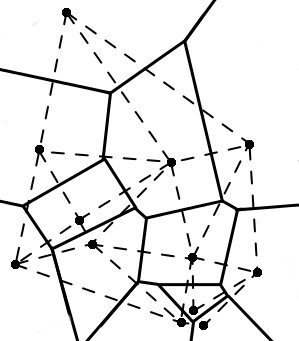
\includegraphics[width=0.75\linewidth]{voronoi}
	\caption{An example Voronoi diagram for objects on a 2-dimensional space.  The black lines correspond to the borders of the Voronoi region, while the dashed lines correspond to the edges of the Delaunay Triangulation.}
	\label{voro-ex}
\end{figure}


With the components of a DHT defined above we can now show the relationship between DHTs and the primal-dual problems of Delaunay Triangulation and Voronoi Tessellation.

We can map a given node's ID to a point in a space and the set of short peers to the Delaunay triangulation.
This would make the range of keys a node is responsible correspond to the node's Voronoi region.
Long peers serve as shortcuts across the mesh formed by Delaunay triangulations.


Thus, if we can calculate the Delaunay triangulation between nodes in a DHT, we have a generalized means of creating the overlay network.
This can be done with any algorithm that calculates the Delaunay Triangulation.

Computing the Delaunay Triangulation and/or the Voronoi Tesselation of a set of points is a well analyzed problem.
Many algorithms exist which efficiently compute a Voronoi tessellation for a given set of points on a plane, such as Fortune's sweep line algorithm \cite{fortune1987sweepline}.

However, DHTs are distributed and many of the algorithms to compute Delaunay Triangulation and/or Delaunay Triangulation are unsuited to a distributed environment.
In addition, the computation cost increases when we move into spaces with greater than two dimensions.
In general, finding the Delaunay Triangulation of $n$ points in a space with $d$ dimensions takes $O(n^{\frac{2d-1}{d}})$ time \cite{watson1981computing}.


Is there an algorithm we can use to efficiently calculate Delaunay Triangulations for a distributed system in an arbitrary space?
We created an algorithm called the Distributed Greedy Voronoi Heuristic (DGVH), explained below \cite{dgvh}.


\subsection{Distributed Greedy Voronoi Heuristic}
\label{sec:dgvh}


The Distributed Greedy Voronoi Heuristic (DGVH) is an efficient method for nodes to define their individual Voronoi region (Algorithm \ref{alg:dgvh}). 
DVGH selects nearby nodes that would correspond to points connected to it within a Delaunay triangulation.
Our previous implementation relied on a midpoint function \cite{dgvh}.
We have refined our heuristic to render a midpoint function unnecessary.

The heuristic is described in Algorithm \ref{alg:dgvh}.
Every maintenance cycle, nodes exchange their peer lists with their short peers.
A node creates a list of candidates by combining their peer lists with their neighbor's peer lists.\footnote{In our previous paper, nodes exchange short peer lists with a single peer. Calls to DGVH in this paper use the information from all their short peers.}
Sort the list of peers from closest to furthest distance.
The node then initializes a new peer list with the closest candidate.
For each of the remaining candidates, the node compares the distance between the current short peers and the candidate.
If the new peer list does not contain any short  peers closer to the candidate than the node, the candidate is added to the new peer list.
Otherwise, the candidate is set aside.

The resulting short peers are a subset of the node's actual Delaunay neighbors.
A crucial feature is that this subset guarantees that DGVH will form a routable mesh.


\begin{algorithm} % make smaller
	\caption{Distributed Greedy Voronoi Heuristic}
	\label{alg:dgvh}
%	\algsetup{linenosize=\tiny}
	\small
	\begin{algorithmic}[1]  % the numberis how many lines
		\State Given node $n$ and its list of $candidates$.
		\State Given the minimum $table\_size$
		\State $short\_peers \leftarrow$ empty set% that will contain $n$'s one-hop peers
		\State $long\_peers \leftarrow$ empty set %that will contain $n$'s peers further than one hop.
		\State Sort $candidates$ in ascending order by each node's \texttt{distance} to $n$
		\State Remove the first member of $candidates$ and add it to $short\_peers$
		\ForAll {$c$ in $candidates$}
			\If{any node in $short\_peers$ is closer to $c$ than $n$}
				\State Reject $c$ as a peer
			\Else
				\State Remove $c$ from $candidates$
				\State Add $c$ to $short\_peers$
			\EndIf
		\EndFor
		\While{$|short\_peers| < table\_size $ and $ |candidates| >0$}
			\State Remove the first entry $c$ from $candidates$
			\State Add $c$ to $short\_peers$
		\EndWhile
		\State Add $candidates$ to the set of $long\_peers$	
		\State \texttt{handleLongPeers}($long\_peers$)
		%\IF{$|long\_peers| > table\_size^2$}
		%	\State $long\_peers \leftarrow$ random subset of $long\_peers$ of size $table\_size^2$
		%\ENDIF
	\end{algorithmic}
\end{algorithm} 


Candidates are gathered via a gossip protocol as well as notifications from close peers.
How long peers are handled depends on the particular DHT implementation.
This process is described more in Section \ref{sec:protocol}.

The expected maximum size of $ candidates $ corresponds to the expected maximum degree of a vertex in a Delaunay Triangulation.
This is  $\Theta(\frac{\log n}{\log \log n} )$, regardless of the number of the dimensions \cite{bern1991expected}. 
We can therefore expect \textit{short peers} to be bounded by $\Theta(\frac{\log n}{\log \log n})$.

The expected worst case cost of DGVH is \(O(\frac{\log^{4} n}{\log^{4} \log n} )\) \cite{dgvh}, regardless of the dimension \cite{dgvh}.\footnote{As mentioned in the previous footnote, if we are exchanging peers with a single neighbor rather than all our neighbors, the cost lowers to \(O(\frac{\log^{2} n}{\log^{2} \log n} )\).}
In most cases, this cost much lower, on the order of $ O(dk\log(k) + k^{2} ) $ for $ d $ dimensions and $ k $ candidates.
Additional details can be found in our previous work \cite{dgvh}.



%TODO Justify euclidea and hyperbolic geometry
We have tested DGVH on Chord (a ring-based topology), Kademlia (an XOR-based tree topology), general Euclidean spaces, and even in a hyperbolic geometry.
This is interesting because not only can we implement the contrived topologies of existing DHTs, but more generalizable topologies like Euclidean or hyperbolic geometries.
We show in Section \ref{sec:experiments} that DGVH works in all of these spaces.
DGVH only needs the following functions to be defined in order for nodes to perform lookup operations and determine responsibility.


\begin{itemize}
	\item \textbf{A \texttt{distance} function } - This measures distance in the overlay formed by the Distributed Hash Table.
	In most DHTs, the distance in the overlay has no correlation with real-world attributes.
	
	\item \textbf{A \texttt{responsibility} definition}  This defines the range of keys a node is responsible for. 
	Not every DHT defines which node is responsible for particular keys in the same way. 
	For example, nodes in Kademlia are responsible for the keys closest to themselves, while in Chord, nodes are responsible for the keys falling between themselves and the preceding node.
\end{itemize}

We will now show how we used this information and algorithms to create UrDHT, our abstract model for  distributed hash tables.




\section{UrDHT}
\label{sec:urdht}


The name of UrDHT comes from the the German prefix \textit{ur}, which means ``original.'' 
Our name states that all DHTs can spring from UrDHT.

UrDHT is divided into 3 broad components: Storage, Networking, and Logic.
Storage handles file storage and Networking dictates the protocol for how nodes communicate.
These components oversee the lower level mechanics of how files are stored on the network and how bits are transmitted through the network.
The specifics are outside the scope of the paper, but can be found on the UrDHT Project site \cite{urdht}.

Most of our discussion will focus on the Logic component.
The Logic component is what dictates the behavior of nodes within the DHT and the construction of the overlay network.
It is composed of two parts: the DHT Protocol and the Space Math.

The DHT Protocol contains the canonical operations that a DHT performs, while the Space Math is what effectively distinguishes one DHT from another.
A developer only needs to change the details of the \texttt{space math} package in UrDHT to create a new type of DHT.
We discuss each in further detail below.

\subsection{The DHT Protocol }
\label{sec:protocol}

The DHT Protocol (\texttt{LogicClass.py}) \cite{urdht} is the shared functionality between every single DHT.
It consists of the node's information, the short peer list that defines the overlay, the long peers that make efficient routing possible, and all the functions that use them.
There is no need for a developer to change anything in the DHT Protocol, but it can be modified if so desired.
The DHT Protocol depends on functions from Space Math in order to perform operations within the specified space.

Many of the function calls should be familiar to anyone who has study DHTs.
We will discuss a few new functions we added and the ones that contribute to node maintenance.


%TODO Further justify lookup
The first thing we note is the absence of \texttt{lookup}.
In our efforts to further abstract DHTs, we have replaced \texttt{lookup} using the function \texttt{seek}.
The \texttt{seek} function acts a single step of \texttt{lookup}.
It returns the closest node to $ key $ that the node knows about.
Nodes can perform \texttt{lookup} by iteratively calling \texttt{seek} until it receives the same answer twice.


The \texttt{join} operation takes in a set of bootstrap nodes, called $ candidates $, rather than a single node.
This is part of our plans about how UrDHT can be used as a bootstrap network by providing bootstrapping information for a particular network.
We expect nodes that want to join a particular network to be able to query UrDHT and receive a list of nodes that they can use to bootstrap the joining.

The joining node randomly selects one of these $ candidates $ and finds the ``parent'' node currently responsible for the space.
The joining node then populates its short peers using the ``parent'' node's short peers.
The node  uses the parent to populate its short peer list and then makes it aware of its existence using \texttt{notify}.
Once that has been finished, the joining node starts its maintenance thread.




Maintenance is done via gossip.
Each maintenance cycle, the node recalculates its Delaunay (short) peers using its neighbor's peer list and any nodes that have notified it since the last maintenance cycle.
This is done using DGVH by default, but could be done with some other algorithm.
Once those are calculated, the node handles modifying its long peers, as dictated by the \texttt{handleLongPeers} function described in Section \ref{sec:space}.

\subsection{The Space Math}
\label{sec:space}
The Space Math consists of the functions that define the DHT's topology.
It requires a way to generate short peers to form a routable overlay and a way to choose long peers.
We use DGVH for generating short peers, which works in every space tested.
Space Math requires the following functions when using DGVH:

\begin{itemize}

%\subsubsection{IDToPoint}
\item The \texttt{idToPoint} function takes in a node's ID and any other attributes needed to map an ID onto a point in the space.

In the vast majority of DHTs, this \texttt{idToPoint} function needs nothing more than the ID as input.
The ID is directly translated into a large integer and used as a coordinate in a one dimensional space.


%\subsubsection{Distance}
\item The \texttt{distance} function takes in two points, $a$ and $b$, and outputs the shortest distance from $a$ to $b$.
This distinction matters since distance is not symmetric in every DHT.
The prime example of this is Chord, which is a unidirectional toroidal ring.



%\subsubsection{Get Closest}
\item The function \texttt{getClosest} returns the point closest to $ center$ from a list of $ candidates$, measured by the distance function.
Depending on what you want to measure, \texttt{getClosest} might measure the distance from $ center$ to each of the candidates or from each of the candidates to the $ center$.

%\subsubsection{Get Delaunay (short) Peers}
\item We use the above functions to implement  \texttt{getDelaunayPeers}.
Given a set of points, the $ candidates$, and a center point $ centers$, \texttt{getDelaunayPeers} calculates a mesh that is made up of the Delaunay peers of $ center$.

We assume that this is done using DGVH, shown by the Python code 
in Listing \ref{lst:dgvh}

%TODO I don't see any minimums here
%TOD Put minimum in here
\begin{lstlisting}[basicstyle=\scriptsize\ttfamily,  breaklines=true, caption={\texttt{getDelaunayPeers()}}, label={lst:dgvh}, frame=single] 
def getDelaunayPeers(candidates,center):    
	if len(candidates) < 2:
		return candidates
	sortedCandidates = sorted(candidates, key=lambda x: distance(x, center))
	peers = [sortedCandidates[0]] 
	sortedCandidates = sortedCandidates[1:]
	for c in sortedCandidates:
		accept = True
		for p in peers:
			if distance(c,p) < distance(c,center):
				accept = False
				break
		if accept:
			peers.append(c)
	return peers
\end{lstlisting}


%\subsubsection{Handle Long Peers}

\item The final function is \texttt{handleLongPeers}.
\texttt{handleLongPeers} takes in a list of $ candidates $ and a $ center$, much like \texttt{getDelaunayPeers}, and returns a set of peers to act as routing shortcuts.


The implementation of this function should vary greatly from one DHT to another.
For example, Symphony \cite{symphony} and other small-world \cite{kleinberg2000navigation} networks choose long peers using a probability distribution.
Chord has a much more structured distribution, with each long peer being increasing powers of 2 distance away from the node \cite{chord}.



%In some case it may more convenient implement \texttt{handleLongPeers} as part of \texttt{getDelaunayPeers}.

\end{itemize}


%\subsubsection*{Put and Poll}
%The functions of \texttt{store} and \texttt{get} can be further abstracted otu to \texttt{put} and \texttt{poll}


%This does X


\section{Implementing other DHTs}
\label{sec:implement}
\subsection{Implementing Chord}

Ring topologies are fairly straightforward since they act as are one dimensional Voronoi tessellations, splitting up what is effectively a modular number line among multiple nodes.

Chord uses a unidirectional distance function.
Given two integer keys $ a $ and $ b $ and a maximum value $ 2^{m} $, the \texttt{distance} from $ a $ to $ b $ in Chord's unidirectional ring is: 
\[ distance(a,b) =
\begin{cases}
	2^m + b - a, & \text{if } b - a < 0 \\
	b-a, & \text{otherwise}
\end{cases}
  \]


Short peer selection is trivial in chord, so rather than using DGVH for \texttt{getDelaunayPeers}, each node chooses  from the list of candidates the candidate closest to it (predecessor) and the candidate it is closest to (successor).

Chord's finger (long peer) selection strategy is emulated by \texttt{handleLongPeers}.
For each of the $i$th bits in the hash function, we choose a long peer $ p_i $ from the candidates such that 

%TODO My mathfu is weak I need help

\[ p_i = \left\{c \in Candidates |  \min\left(distance(c, t_{i})\right) \right\}  \]
where
\[t_{i} =  (n + 2^{i}) \mod 2^m \]
for the current node $n$.

%for i in range(0, HASHBASE):
%target = tuple([(center[0] + 2**i) % HASHMAX])
%subject = min(others, key=lambda x: chordDist(x.loc, target))
%We know Chord's invariants are not (citation), but our protocol isn't affected by these constraints


\subsection{Implementing Kademlia}
Kademlia uses the exclusive or, or XOR, metric for distance.
This metric, while non-euclidean, is perfectly acceptable for calculating distance in Kademlia \cite{kademlia}.
For two given keys $ a $ and $ b $

\[ disance(a, b) = a  \oplus b\]

The \texttt{getDelaunayPeers} function uses DGVH as normal to choose the short peers for node $n$.
We then used Kademlia's $k$-bucket strategy \cite{kademlia} for \texttt{handleLongPeers}.
The remaining candidates are placed into buckets, each capable holding a maximum of $k$ long peers.

To summarize briefly, node $n$ starts with a single bucket containing $n$, covering long peers for the entire range.
When attempting to add a candidate to a bucket already containing $k$ long peers, if the bucket contains node $n$, the bucket is split into two buckets, each covering half of that buckets range.
Further details of how Kademlia $k$-buckets work can be found in the Kademlia protocol paper \cite{kademlia}.


\subsection{ZHT}
ZHT \cite{li2013zht} leads to an extremely trivial implementation in UrDHT.
Unlike other DHTs, ZHT assumes an extremely low rate of churn.
It bases this rationale on the fact that tracking $ O(n) $ peers in memory is trivial.
This indicates the $ O( \log n)  $  memory  requirement for other DHTs is overzealous and not based on a memory limitation.
Rather, the primary motivation for keeping a limited subset of the network in memory is more due to the cost of maintenance messages.
ZHT shows, that by assuming low rates of churn (and infrequent maintenance messages as a result), having $O(n)$ peers is a viable tactic for faster lookups.

As a result, the topology of ZHT is a clique, with each node having an edge to all other nodes, yielding $ O(1) $ lookup times with an $ O(n) $ memory cost.
%
The only change that needs to be made is to consider all peer candidates to be short peers.

\subsection{Implementing a DHT in a non-contrived Metric Space}

We used a Euclidean geometry as the default space when building UrDHT and DGVH \cite{dgvh}.
For two vectors $\vec{a}$ and $\vec{b}$ in $d$ dimensions: 

\[distance\left(\vec{a}, \vec{b}\right) = \sqrt{\sum\limits_{i\in d} \left(a_i-b_i\right)^2}\]


We implement \texttt{getDelaunayPeers} using DGHV and set the minimum number of short peers to $3d+1$, a value we found through experimentation \cite{dgvh}.

Long peers are randomly selected from the left-over candidates after DGVH is performed \cite{dgvh}.
The maximum size of long peers is set to $(3d+1)^2$, but it can be lowered or eliminated if desired and maintain $ O(\sqrt[d]{n}) $ routing time.


Generalized spaces such as Euclidean space allow the assignment of meaning to arbitrary dimension and allow for the potential for efficient querying of a database stored in a DHT.

%\subsection{Implementing a DHT in a Hyperbolic Geometry}
	
\label{sec:hyper}

We have already shown with Kademlia that UrDHT can operate in a non-Euclidean geometry.
Another non-euclidean geometry UrDHT can work in is a hyperbolic geometry.

We implemented a DHT within a hyperbolic geometry using a Poincar\`{e} disc model.
To do this, we implemented \texttt{idToPoint} to create a random point in Euclidean space from a uniform distribution.
This point is then mapped to a Poincar\`{e} disc model to determine the appropriate Delaunay peers.
For any two given points $a$ and $b$ in a Euclidean vector space, the \texttt{distance} in the  Poincar\`{e} disc is:


\[ distance(a, b) = \operatorname{arcosh} \left(  1+ 2 \frac{ \left\| a - b \right\| ^{2} }{ ( 1 - \left\| a \right\| ^{2} ) ( 1 - \left\| b \right\| ^{2} ) }\right) \]


Now that we have a \texttt{distance} function, DGVH can be used in \texttt{getDelaunayPeers} to generate an approximate Delaunay Triangulation for the space.
The \texttt{getDelaunayPeers} and \texttt{handleLongPeers} functions are otherwise implemented exactly as they were for Euclidean spaces. 




Implementing a DHT in hyperbolic geometry has many interesting implications.
Of particular note, embedding into hyperbolic spaces allows us to explore accurate embeddings of internode latency into the metric space \cite{kleinberg2007geographic} \cite{cvetkovski2009hyperbolic}.
This has the potential to allow for minimal latency DHTs.


%\subsection{Services}
%
%There needs to be an easy way to append data to the bootstrapping list.
%
%To do this, we introduce the \texttt{put} and  \texttt{poll} primitives.
%These functions can considered abstracted versions.
%	
\section{Experiments}
\label{sec:experiments}

We use simulations to test our implementations of DHTs using UrDHT.
Using simulations to test the correctness and relative performance of DHTs is standard practice for testing and analyzing DHTs \cite{kademlia} \cite{chord} \cite{tapestry} \cite{symphony} \cite{raynet} \cite{li2005comparing}.

Our experiments demonstrate that topologies implemented using UrDHT converge to a routable mesh.
We demonstrate that lookup operations in these meshes can be done in sublinear time.

Tests
k connected randomly populated network
vars:
k for your k connected network 10, 20
duration what we have works
size 100, 500, 1000, 5000 if possible,

Iterative joins, start with one node
vars:  join rate (ticks per join) ,1 3 
final size  100, 500, 1000, 5000 if possible,
join method (bootstrapping size)  all,

outputs
Network diameter at tick
avg greedy routing distance
greedy routing success rate at tick
maximum degree
mean degree
std deviatation degree
Anything we want for degree


Graph max degree vs expected  maximimum degree  (this is short peers)



\subsection{Kademlia Works}
B


\subsection{Performance of Chord on our network module}



\subsection{UrDHT Cohesion Euclidean Space}
This experiment greatly resembles the one we performed when evaluating DGVH \cite{dgvh}.

We've previously shown that higher degrees work \cite{dgvh}.

\subsection{Cohesion in hyperbolic space}
We showed in worked in DGVH, it should work in a hyperbolic space.




%\subsection{Remarks}
%Our experiments show that Euclidean and Hyperbolic topologies offer a distinct advantage over Chord and Kademlia.
%Chord and Kademlia cannot create a organized network from an initially randomly connected graph.
%Because Chord and Kademlia are highly selective in what they select in long peers, this first pass culling reduces the initially connected graph into multiple disjoint sets from which it cannot recover.
%
%We have demonstrated here and in our previous works that DHTs in Euclidean and Hyperbolic topologies can converge from a randomized topology. 
%This means so long as the graph is connected

%With an initial $k$-connected graph, the first step is for nodes to select short and long peers.

\section{Applications and Future Work}
\label{sec:future}

%Restate the intro
UrDHT is a unified model for DHTs and framework for building distributed applications.

Future improvements of UrDHT would further disconnect long peers and short peers giving them their own implementation cycle.

%Future stuff
There are numerous routes we can take with our model.
Of particular interest are the applications of building a DHT overlay that operates in a hyperbolic geometry.

One of the other features shared by nearly every DHT is that routing works by minimizing the number of hops across the overlay network, with all hops treated as the same length.
This is done because it is assumed that DHTs know nothing about the state of actual infrastructure the overlay is built upon.

However, this means that most DHTs will happily route a message from one continent to another and back.
This is obviously undesirable, but it is the status quo in DHTs.
This stems from the generation of node IDs in DHTs. 
Nodes are typically assigned a point in the range of a cryptographic hash function. 
This ID corresponds to the hash of some identifier or given a point randomly.
This is done for purposes of load balancing and fault tolerance.

We want to see if there is a means of embedding latency into the DHT, while still maintaining the system's fault tolerance.
Doing so would mean that the hops traversed to a destination are, in fact, the shortest path to the destination.

We believe we can embed a latency graph in a hyperbolic space and define UrDHT such that it operates within this space.
The end result would be a DHT with latency embedded into the overlay.
Nodes would respond to changes in latency and the network by rejoining the network at new positions.
%We use  a force spring model to accomplish this.



%Hyperbolic spaces allow us to cleanly embed scale free graphs

\bibliography{mine,dht,voronoi}
\bibliographystyle{IEEEtran}

\end{document}
